% mnras_template.tex 
%
% LaTeX template for creating an MNRAS paper
%
% v3.0 released 14 May 2015
% (version numbers match those of mnras.cls)
%
% Copyright (C) Royal Astronomical Society 2015
% Authors:
% Keith T. Smith (Royal Astronomical Society)

% Change log
%
% v3.2 July 2023
%	Updated guidance on use of amssymb package
% v3.0 May 2015
%    Renamed to match the new package name
%    Version number matches mnras.cls
%    A few minor tweaks to wording
% v1.0 September 2013
%    Beta testing only - never publicly released
%    First version: a simple (ish) template for creating an MNRAS paper

%%%%%%%%%%%%%%%%%%%%%%%%%%%%%%%%%%%%%%%%%%%%%%%%%%
% Basic setup. Most papers should leave these options alone.
\documentclass[fleqn,usenatbib]{mnras}

% MNRAS is set in Times font. If you don't have this installed (most LaTeX
% installations will be fine) or prefer the old Computer Modern fonts, comment
% out the following line
\usepackage{newtxtext,newtxmath}
% Depending on your LaTeX fonts installation, you might get better results with one of these:
%\usepackage{mathptmx}
%\usepackage{txfonts}

% Use vector fonts, so it zooms properly in on-screen viewing software
% Don't change these lines unless you know what you are doing
\usepackage[T1]{fontenc}

% Allow "Thomas van Noord" and "Simon de Laguarde" and alike to be sorted by "N" and "L" etc. in the bibliography.
% Write the name in the bibliography as "\VAN{Noord}{Van}{van} Noord, Thomas"
\DeclareRobustCommand{\VAN}[3]{#2}
\let\VANthebibliography\thebibliography
\def\thebibliography{\DeclareRobustCommand{\VAN}[3]{##3}\VANthebibliography}


%%%%% AUTHORS - PLACE YOUR OWN PACKAGES HERE %%%%%

% Only include extra packages if you really need them. Avoid using amssymb if newtxmath is enabled, as these packages can cause conflicts. newtxmatch covers the same math symbols while producing a consistent Times New Roman font. Common packages are:
\usepackage{graphicx}	% Including figure files
\usepackage{amsmath}	% Advanced maths commands
\usepackage{tikz}
\usetikzlibrary{graphs,shapes.geometric}

%%%%%%%%%%%%%%%%%%%%%%%%%%%%%%%%%%%%%%%%%%%%%%%%%%

%%%%% AUTHORS - PLACE YOUR OWN COMMANDS HERE %%%%%

% Please keep new commands to a minimum, and use \newcommand not \def to avoid
% overwriting existing commands. Example:
%\newcommand{\pcm}{\,cm$^{-2}$}	% per cm-squared
\newcommand{\eep}{\ensuremath{\mathrm{EEP}}}
\newcommand{\feh}{\ensuremath{\mathrm{[Fe/H]}}}
\newcommand{\normal}{\mathcal{N}}
\newcommand{\uniform}{\mathcal{U}}
\renewcommand*{\vec}[1]{\boldsymbol{#1}}

%%%%%%%%%%%%%%%%%%%%%%%%%%%%%%%%%%%%%%%%%%%%%%%%%%

%%%%%%%%%%%%%%%%%%% TITLE PAGE %%%%%%%%%%%%%%%%%%%

% Title of the paper, and the short title which is used in the headers.
% Keep the title short and informative.
\title[Scalable stellar inference]{[TBC] Scalable stellar inference: hierarchical Bayesian framework with a neural network surrogate model for stellar evolution}

% The list of authors, and the short list which is used in the headers.
% If you need two or more lines of authors, add an extra line using \newauthor
\author[A. J. Lyttle et al.]{
Alexander J. Lyttle,$^{1}$\thanks{E-mail: a.j.lyttle@bham.ac.uk (AJL)}
Guy R. Davies,$^{1}$
and TBC
\\
% List of institutions
$^{1}$School of Physics and Astronomy, University of Birmingham, Birmingham B15 2TT, UK
}

% These dates will be filled out by the publisher
\date{Accepted XXX. Received YYY; in original form ZZZ}

% Enter the current year, for the copyright statements etc.
\pubyear{2024}

% Don't change these lines
\begin{document}
\label{firstpage}
\pagerange{\pageref{firstpage}--\pageref{lastpage}}
\maketitle

% Abstract of the paper
\begin{abstract}

\end{abstract}

% Select between one and six entries from the list of approved keywords.
% Don't make up new ones.
\begin{keywords}
methods: statistical -- stars: fundamental parameters -- stars: low-mass
\end{keywords}

%%%%%%%%%%%%%%%%%%%%%%%%%%%%%%%%%%%%%%%%%%%%%%%%%%

%%%%%%%%%%%%%%%%% BODY OF PAPER %%%%%%%%%%%%%%%%%%

\section{Introduction}

Here is an example citation in text \citet{Lyttle.Davies.ea2021} and in parentheses \citep{Lyttle.Davies.ea2021}.

\section{Methods}
\label{sec:methods}

\subsection{Hierarchical Bayesian model}
\label{sec:hbm}

\begin{equation}
    p(\vec{\theta}, \phi \mid \vec{d}) \propto p(\vec{d} \mid \vec{\theta}) \, p(\vec{\theta} \mid \phi) \, p(\phi),
\end{equation}

\begin{equation}
    \begin{split}
        p(\theta_i \mid \phi) &= \normal(Y_i \mid a_Y + b_Y Z_i, \sigma_Y^2) \, \normal(\alpha_i \mid \mu_\alpha, \sigma_\alpha^2) \\
        &\times p(\eep_i, M_i, \feh_i)
    \end{split}
\end{equation}

\begin{equation}
    \begin{split}
        p(\phi) &= \normal(a_Y \mid 0.247, 0.001) \, \uniform(b_Y \mid 0.0, 3.0) \\
        &\times \normal(\ln \sigma_Y \mid x.xx, x.xx) \, \uniform(\mu_\alpha \mid 1.5, 2.5) \\
        &\times \normal(\ln \sigma_\alpha \mid x.xx, x.xx)
    \end{split}
\end{equation}

\begin{figure}
    \centering
    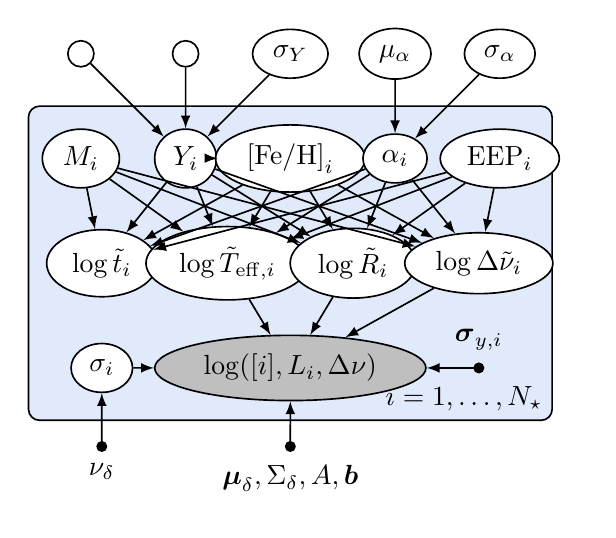
\begin{tikzpicture}[scale=1.33, line width=0.6pt, every node/.style={ellipse, draw, fill=white}, >=latex]
    % Hyperparameters
    \node (ay) at (0, 5) {$\yp$};
    \node (by) at (1, 5) {$\dydz$};
    \node (sy) at (2, 5) {$\sigma_Y$};
    \node (ma) at (3, 5) {$\mu_\alpha$};
    \node (sa) at (4, 5) {$\sigma_\alpha$};

    % Plate - Individual star
    \draw[fill=CornflowerBlue!20, rounded corners] (-0.5, 1.5) rectangle (4.5, 4.5);
    % \draw[fill=JungleGreen!20, rounded corners] (-0.5, 1.5) rectangle (4.5, 4.5);
    % \node[draw=none, fill=none, rotate=90, above, align=left, anchor=south west] at (-0.5, 1.5) {Individual\\Star};
    \node[draw=none, fill=none, above left, align=right] at (4.5, 1.5) {$i = 1, \dots, N_\star$};

    % Input parameters
    \node (mi) at (0, 4) {$M_i$};
    \node (yi) at (1, 4) {$Y_i$} edge [<-] (ay) edge [<-] (by) edge [<-] (sy);
    \node (fehi) at (2, 4) {$\feh_i$} edge [->] (yi);
    \node (ai) at (3, 4) {$\alpha_i$} edge [<-] (ma) edge [<-] (sa);
    \node (eepi) at (4, 4) {$\eep_i$};

    % Output parameters
    % \node (age) at (0, 3) {$t_i$};
    % \node [fill=black!25] (teff) at (1, 3) {$T_{\mathrm{eff}, i}$};
    % \node [fill=black!25] (lum) at (2, 3) {$L_i$} edge [<-] (teff);
    % \node (rad) at (3, 3) {$R_i$} edge [->] (lum);
    % \node (dnu) at (4, 3) {$\Delta\nu_i$};
    \node (age) at (0.2, 3) {$\log \tilde t_i$};
    \node (teff) at (1.4, 3) {$\log \tilde T_{\mathrm{eff}, i}$};
    \node (rad) at (2.6, 3) {$\log \tilde R_i$};
    \node (dnu) at (3.8, 3) {$\log \Delta\tilde\nu_i$};

    % Connect neural network inputs and outputs
    \foreach \x in {mi, yi, fehi, ai, eepi}
    \foreach \y in {age, teff, rad, dnu}
    \draw[->] (\x) -- (\y);

    \node [fill=black!25] (obs) at (2, 2) {$\log(\teff[i], L_i, \Delta\nu)$} edge [<-] (teff) edge [<-] (rad) edge [<-] (dnu);
    % Plate - Emulator noise
    % \draw[fill=BurntOrange!20, rounded corners] (-0.5, 0.4) rectangle (1.5, 1.4);
    % \node[draw=none, fill=none, rotate=90, above, align=left, anchor=south west] at (-0.5, 0.4) {Emulator\\Error};
    % \node[draw=none, fill=none, above left, align=right] at (1.5, 0.4) {$j = 1, \dots, N_\mathrm{out}$};

    % Emulator uncertainty
    % \node (sig) at (1, 0.9) {$\sigma_j$} edge [->] (teff) edge [->] (lum);
    % \fill (0, 0.9) circle (1.5pt) edge [->] (sig) node[above, fill=none, draw=none] (slum) {$\tau_j$};
    % \fill (2, 0.9) circle (1.5pt) edge [->] (sig) node[above, fill=none, draw=none] (slum) {$\nu$};

    % \node (sig) at (1, 1) {$u$} edge [->] (teff) edge [->] (lum);
    % \fill (0, 1) circle (1.5pt) edge [->] (sig) node[above, fill=none, draw=none] (slum) {$\nu, \vec{\tau}$};

    % \node (sig) at (1, 2) {$\Sigma_i$} edge [->] (teff) edge [->] (lum);

    % \node (sig) at (1, 2) {$\mat\Sigma_i$} edge [->] (obs);

    \node (sig) at (0.2, 2) {$\sigma_i$} edge [->] (obs);

    % \fill (1, 1) circle (1.5pt) edge [->] (sig) node[right, fill=none, draw=none] (slum) {$\nu, \vec{\tau}$};

    % Observational Uncertainty
    % \fill (0, 2) circle (1.5pt) edge [->] (sig) node[below, fill=none,draw=none] {$\sigma_{T_\mathrm{eff}, i}$};
    % \fill (2, 2) circle (1.5pt) edge [->] (sig) node[below, fill=none, draw=none] {$\sigma_{L, i}$};
    
    % \fill (0, 2) circle (1.5pt) edge [->] (sig) node[below, fill=none,draw=none] {$\sigma_{z, i}$};
    % \fill (1, 1) circle (1.5pt) edge [->] (sig) node[below, fill=none,draw=none] {$\nu_\delta, \mat\Sigma_\delta$};
    % \fill (2, 1) circle (1.5pt) edge [->] (obs) node[below, fill=none,draw=none] {$\vec\mu_\delta$};
    
    \fill (3.8, 2) circle (1.5pt) edge [->] (obs) node[above, fill=none,draw=none] {$\vec\sigma_{y, i}$};
    \fill (2, 1.25) circle (1.5pt) edge [->] (obs) node[below, fill=none,draw=none] {$\vec\mu_\delta, \mat\Sigma_\delta, \mat A, \vec b$};
    \fill (0.2, 1.25) circle (1.5pt) edge [->] (sig) node[below, fill=none,draw=none] {$\nu_\delta$};

    % \draw [decorate,decoration={brace,amplitude=4pt}]
    % (4.66, 5.25) -- (4.66, 4.75) node[fill=none,draw=none,midway,right]{$\vec\phi$};
    % \draw [decorate,decoration={brace,amplitude=4pt}]
    % (4.66, 4.25) -- (4.66, 3.75) node[fill=none,draw=none,midway,right]{$\inputs_i$};
    % \draw [decorate,decoration={brace,amplitude=4pt}]
    % (4.66, 3.25) -- (4.66, 2.75) node[fill=none,draw=none,midway,right]{$\pred_i$};

\end{tikzpicture}

    \caption{A probabilistic directed acyclic graph showing the relationship between parameters in the model. Arrows show the direction of dependence. Parameters surrounded by a solid and dotted lines are probabilistic and deterministic respectively. Parameters shaded grey are observed and those shaded black are fixed. Dashed lines group parameters which are inputs to or outputs from other routines (e.g. the neural network). The blue and orange boxes group parameters which loop over \(i\) and \(\zeta\) respectively. Definitions of the parameters and their description are given in the text.}
\end{figure}

\subsection{Stellar model emulator}
\label{sec:emulator}

\subsection{Synthetic stars}
\label{sec:synth}

\section{Results}
\label{sec:results}

\section{Discussion}
\label{sec:discussion}

\section{Conclusion}
\label{sec:conclusion}

\section*{Acknowledgements}

The Acknowledgements section is not numbered. Here you can thank helpful
colleagues, acknowledge funding agencies, telescopes and facilities used etc.
Try to keep it short.

%%%%%%%%%%%%%%%%%%%%%%%%%%%%%%%%%%%%%%%%%%%%%%%%%%
\section*{Data Availability}
 
The inclusion of a Data Availability Statement is a requirement for articles published in MNRAS. Data Availability Statements provide a standardised format for readers to understand the availability of data underlying the research results described in the article. The statement may refer to original data generated in the course of the study or to third-party data analysed in the article. The statement should describe and provide means of access, where possible, by linking to the data or providing the required accession numbers for the relevant databases or DOIs.

%%%%%%%%%%%%%%%%%%%% REFERENCES %%%%%%%%%%%%%%%%%%

% The best way to enter references is to use BibTeX:

\bibliographystyle{mnras}
\bibliography{references} % if your bibtex file is called example.bib

% Alternatively you could enter them by hand, like this:
% This method is tedious and prone to error if you have lots of references
%\begin{thebibliography}{99}
%\bibitem[\protect\citeauthoryear{Author}{2012}]{Author2012}
%Author A.~N., 2013, Journal of Improbable Astronomy, 1, 1
%\bibitem[\protect\citeauthoryear{Others}{2013}]{Others2013}
%Others S., 2012, Journal of Interesting Stuff, 17, 198
%\end{thebibliography}

%%%%%%%%%%%%%%%%%%%%%%%%%%%%%%%%%%%%%%%%%%%%%%%%%%

%%%%%%%%%%%%%%%%% APPENDICES %%%%%%%%%%%%%%%%%%%%%

\appendix

%%%%%%%%%%%%%%%%%%%%%%%%%%%%%%%%%%%%%%%%%%%%%%%%%%

% Don't change these lines
\bsp	% typesetting comment
\label{lastpage}
\end{document}

% End of mnras_template.tex
